
Results are presented in four layers, each addressing one experimental question from Section 4.

\subsubsection{Primary Result: Both Metrics at Chance Level}

\begin{figure}[htbp]
\centering
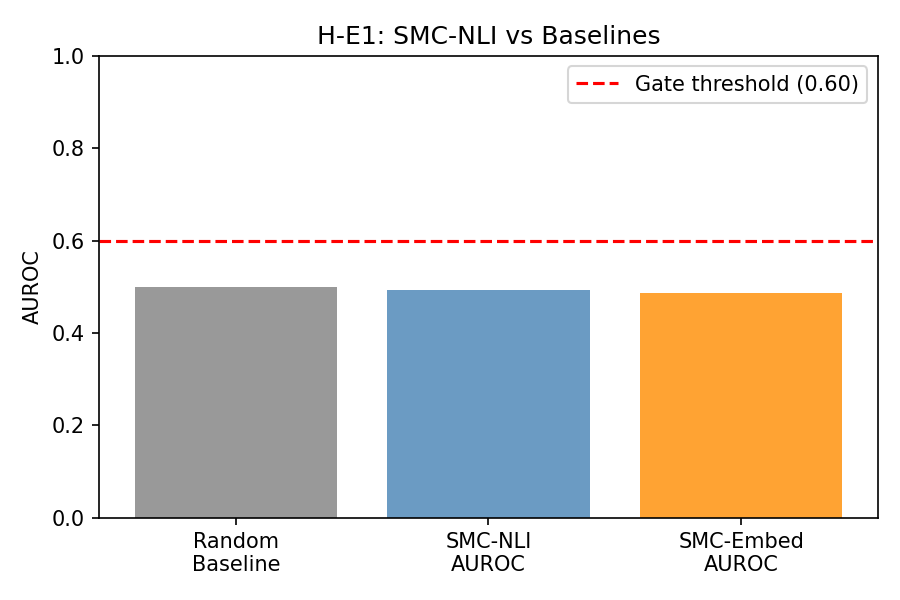
\includegraphics[width=\columnwidth]{figures/auroc_comparison.png}
\caption{AUROC Comparison}
\label{fig:auroc_comparison}
\end{figure}

\textbf{Figure 1.} AUROC comparison across SMC-NLI, SMC-Embed, and the random baseline.

\begin{table}[htbp]
\centering
\resizebox{\columnwidth}{!}{%
\begin{tabular}{llll}
\toprule
Metric & AUROC & Target & Status \\
\midrule
SMC-NLI & **0.4933** & >0.60 & FAIL \\
SMC-Embed & **0.4859** & >0.60 & FAIL \\
Random baseline & 0.50 & --- & --- \\
\bottomrule
\end{tabular}
}
\end{table}

Both SMC-NLI (AUROC=0.4933) and SMC-Embed (AUROC=0.4859) are statistically indistinguishable from a random classifier (AUROC=0.50). Both are substantially below the MUST\_WORK gate threshold of 0.60. A system using SMC-NLI to filter Llama-3-8B-Instruct outputs on HaluEval QA would achieve no improvement over random selection.

\subsubsection{ROC Curve Analysis}

\begin{figure}[htbp]
\centering
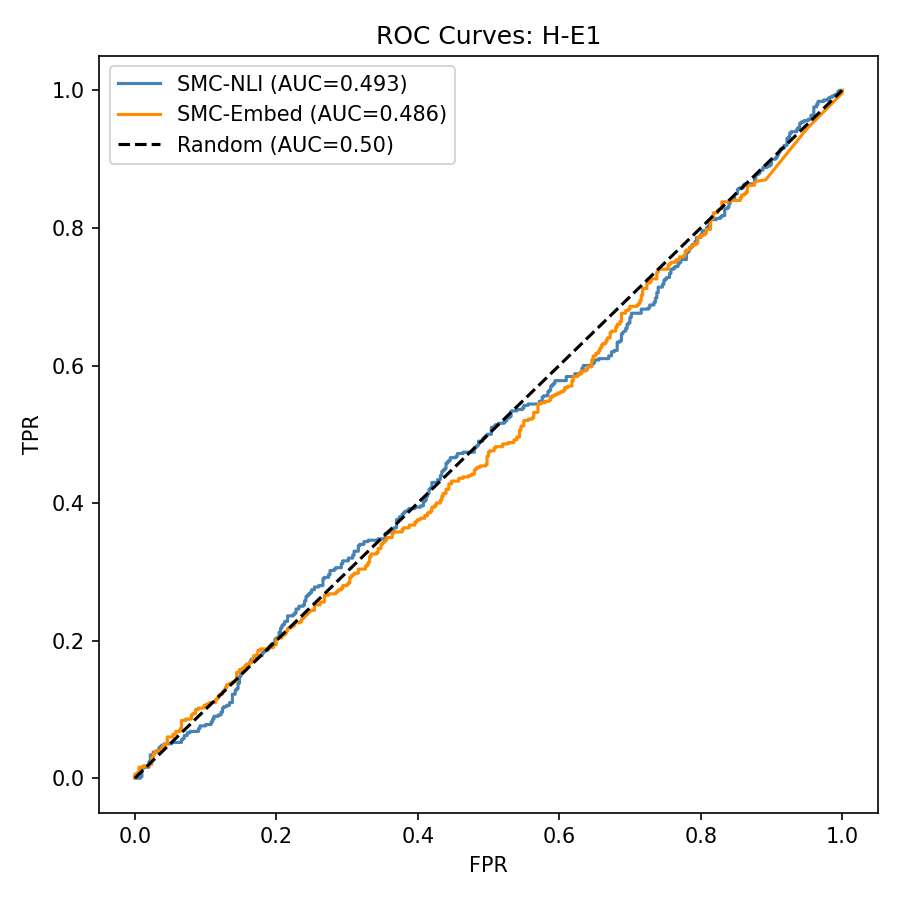
\includegraphics[width=\columnwidth]{figures/roc_curves.png}
\caption{ROC Curves}
\label{fig:roc_curves}
\end{figure}

\textbf{Figure 2.} ROC curves for SMC-NLI and SMC-Embed across all decision thresholds.

Both ROC curves are near-diagonal, confirming that the chance-level AUROC is not an artifact of threshold selection. There is no operating point at which either metric achieves a meaningful sensitivity-specificity trade-off. The curves for SMC-NLI and SMC-Embed nearly overlap, suggesting a shared failure mode.

\subsubsection{Mechanism Analysis: Score Distribution by Label}

\begin{figure}[htbp]
\centering
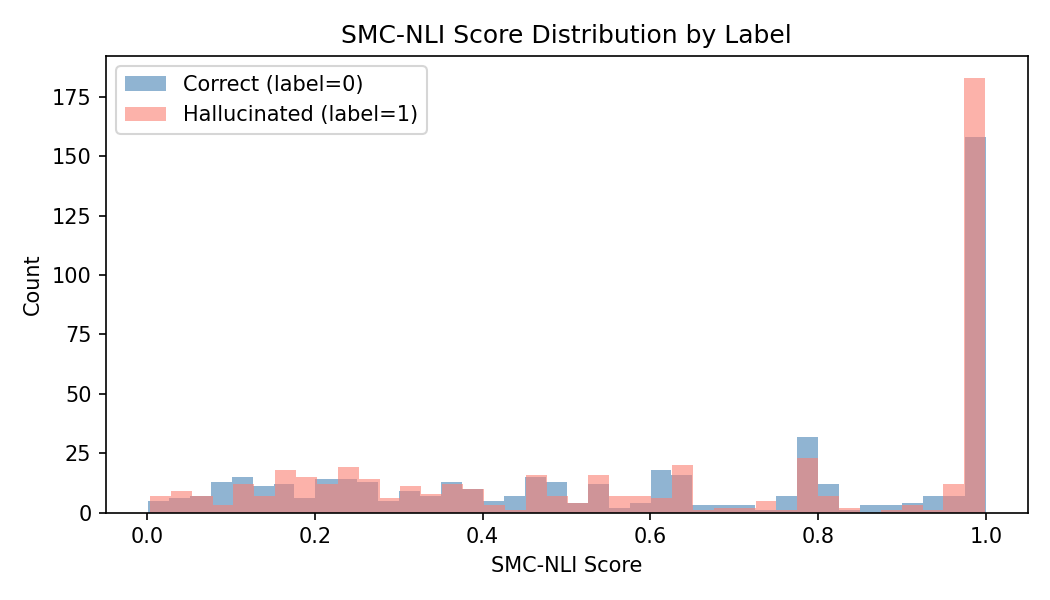
\includegraphics[width=\columnwidth]{figures/smc_nli_distribution.png}
\caption{SMC-NLI Score Distribution}
\label{fig:smc_nli_distribution}
\end{figure}

\textbf{Figure 3.} Distribution of SMC-NLI scores split by HaluEval label (correct vs. hallucinated).

\begin{table}[htbp]
\centering
\resizebox{\columnwidth}{!}{%
\begin{tabular}{ll}
\toprule
Label & Mean SMC-NLI \\
\midrule
Correct (n=500) & **0.6236** \\
Hallucinated (n=500) & **0.6299** \\
Gap & **0.006** \\
Overall std & **0.3388** \\
\bottomrule
\end{tabular}
}
\end{table}

The overall SMC-NLI standard deviation is 0.3388 --- well above the 0.05 threshold, confirming that scores vary meaningfully across questions. The mechanism produces a signal. However, the signal carries no information about the label.

The per-label distributions overlap almost completely. The mean SMC-NLI score for correctly-labeled questions (0.6236) is essentially identical to hallucinated-labeled questions (0.6299), with a gap of 0.006. The direction is also inverted from the theoretical prediction: hallucinated questions show slightly higher consistency (0.6299 > 0.6236), though this difference is not statistically meaningful given N=1000.

The mechanism assumption --- that hallucinated outputs produce lower consistency than correct outputs --- is empirically falsified for this model-task combination. Both label categories produce similarly high-consistency outputs, indicating that Llama-3-8B-Instruct is ''confidently consistent'' regardless of factual accuracy.

\subsubsection{Mechanism Verification: Local vs. Global}

The 5-question mechanism verification passed:

\begin{verbatim}
Q: "What year was the composed of Lux Aurunque born?"       SMC-NLI: 0.9530 | Label: 0 (correct)
Q: "What is the birthdate of this monarch of three...?"     SMC-NLI: 0.3875 | Label: 1 (hallucinated)
Q: "What US Air Force installation was last...?"             SMC-NLI: 0.9853 | Label: 0 (correct)
Q: "Esther Norma Arrostito is a founder of a...?"           SMC-NLI: 0.6162 | Label: 1 (hallucinated)
Q: "What is the birthdate of this American actor...?"       SMC-NLI: 0.4881 | Label: 1 (hallucinated)
Mechanism verification PASSED (range: 0.3875–0.9853, all in [0,1])
\end{verbatim}

The mechanism check shows SMC-NLI varies substantially across 5 questions and appears directionally correct locally (e.g., question 1: high consistency, label=correct; question 2: lower consistency, label=hallucinated). This local appearance is misleading: across 1,000 questions, the discriminative signal collapses to AUROC=0.4933.

This juxtaposition --- local mechanism functioning, global discriminative failure --- is the defining characteristic of the systematic confabulation regime. The scorer works correctly; the assumed population-level signal does not exist.

\subsubsection{Dual-Metric Correlation Analysis}

\begin{figure}[htbp]
\centering
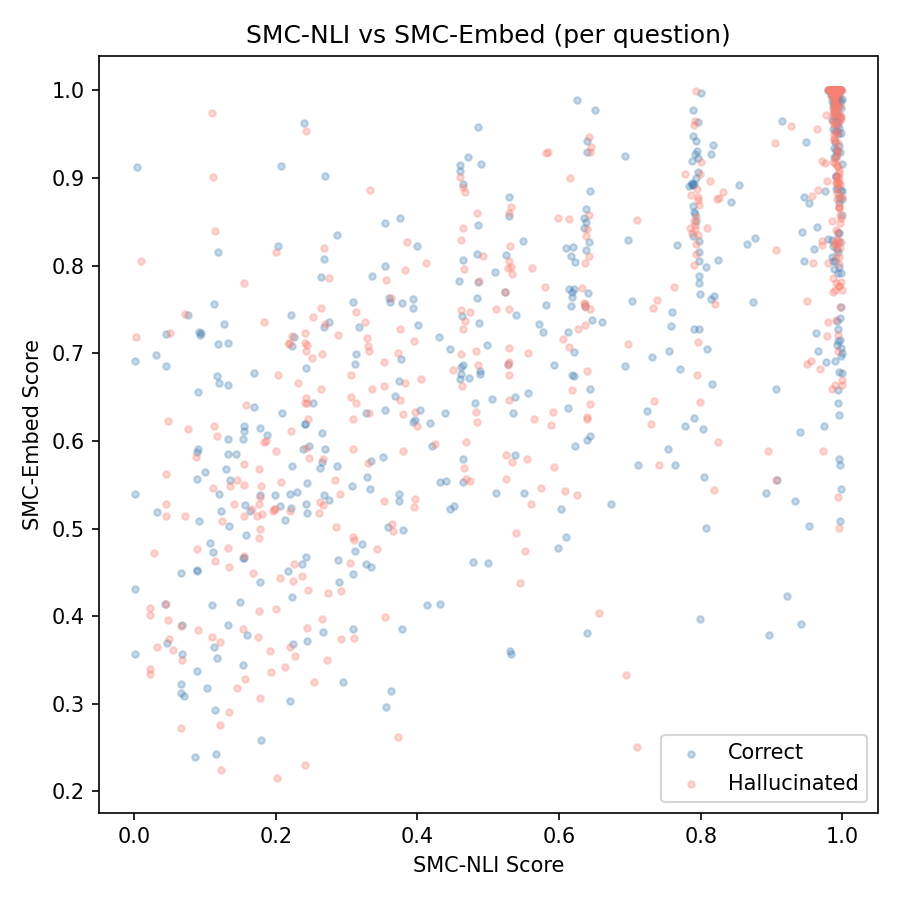
\includegraphics[width=\columnwidth]{figures/nli_vs_embed_scatter.png}
\caption{NLI vs. Embed Scatter}
\label{fig:nli_vs_embed_scatter}
\end{figure}

\textbf{Figure 4.} Per-question SMC-NLI vs. SMC-Embed scatter, confirming the shared failure mode.

The two metrics are strongly correlated across questions: questions with high NLI consistency also tend to have high embedding consistency. This correlation confirms that SMC-NLI and SMC-Embed are measuring the same underlying property --- the output consistency of Llama-3-8B-Instruct --- and that this property is uniformly present regardless of factual accuracy.

The equal failure of both metrics, and their high correlation, is the strongest evidence for the regime-level interpretation: the failure is not in how consistency is measured (NLI vs. embedding) but in whether consistency discriminates labels in this model-task combination.

\subsubsection{Implementation Validation Summary}

\begin{table}[htbp]
\centering
\resizebox{\columnwidth}{!}{%
\begin{tabular}{ll}
\toprule
Check & Result \\
\midrule
Unit tests & 14/14 pass \\
Mechanism verification & PASSED \\
Coder-Validator cycles & 1/5 \\
Total tasks completed & 15/15 \\
LLM samples generated & 10,000 \\
NLI pairs scored & 45,000 \\
\bottomrule
\end{tabular}
}
\end{table}

All implementation checks pass. The negative AUROC result is not attributable to implementation error.

\subsubsection{Summary of Results}

\begin{table}[htbp]
\centering
\resizebox{\columnwidth}{!}{%
\begin{tabular}{ll}
\toprule
Question & Answer \\
\midrule
Q1: Does SMC-NLI achieve AUROC>0.60? & No (AUROC=0.4933) \\
Q2: Does SMC-Embed rule out NLI OOD? & Yes (SMC-Embed=0.4859, equal failure) \\
Q3: Is implementation correct? & Yes (14/14 tests, mechanism check passes) \\
Q4: What does the distribution reveal? & Mechanism failure (gap=0.006, distributions overlap completely) \\
\bottomrule
\end{tabular}
}
\end{table}

The results consistently point to a single interpretation: Llama-3-8B-Instruct on HaluEval QA operates in the systematic confabulation regime, producing consistent outputs for both correct and incorrect beliefs and eliminating the discriminative signal that SMC-based methods require.

